\documentclass{beamer}
\usepackage{beamerthemeshadow}
\usepackage[utf8]{inputenc}
\usepackage[T1]{fontenc}
\usepackage{tikz}
\usepackage{cmbright}
\usepackage{mhchem}
\usepackage{braket}
\usepackage{biblatex}
\usepackage{circuitikz}
\addbibresource{slide_cite_faculty.bib}
\fontencoding{OT1}\fontfamily{cmbr}\selectfont %to load ot1cmbr.fd
\DeclareFontShape{OT1}{cmbr}{bx}{n}{% change bx definition
<->cmbrbx10%
}{}
\normalfont % back to normalfont

\setbeamertemplate{navigation symbols}{}
\setbeamertemplate{section in toc}[sections numbered]
\setbeamertemplate{subsection in toc}[subsections numbered]
\setbeamertemplate{footline}[frame number]
%
\setbeamertemplate{caption}{\raggedright\insertcaption\par}

\newcommand\Fontvi{\fontsize{8}{7.2}\selectfont} %font size changer

%font type:
\newenvironment{ppl}{\fontfamily{ppl}\selectfont}{\par}

\setbeamertemplate{itemize item}{$\blacktriangleright$}

% macros:
\def\D{\displaystyle}
\def\att{                    % mark at the margin
        \marginpar[ \hspace*{\fill} \raisebox{-0.2em}{\rule{2mm}{1.2em}} ]
        {\raisebox{-0.2em}{\rule{2mm}{1.2em}} }
        }
\def\at#1{[*** \att #1 ***]}  % text needing attention
\def\spc{\hspace*{0.5cm}} 			% indentation


%Information to be included in the title page:
\title{Bonding features for H$_x$O$_y$ potential energy surface}
\author[Aribowo, Neumaier] % (optional, for multiple authors)
{Beryl Ramadhian Aribowo}

\institute[VFM] % (optional)
{
    Joint work with Prof. Arnold Neumaier\\
    Faculty of Mathematics\\
    University of Vienna \\

}

%\date[VGSCO 2021] % (optional)
\date[]{VGSCO Retreat \\ June 12, 2022}


\begin{document}

\frame{\titlepage}

\begin{frame}
    \frametitle{Outline}
    \begin{columns}[t]
        \begin{column}{.5\textwidth}
            \tableofcontents[sections={1-2}]
        \end{column}
        \begin{column}{.5\textwidth}
            \tableofcontents[sections={3-5}]
        \end{column}
    \end{columns}
\end{frame}


\section{Pair potential review}
\subsection{Pair potential review}
\begin{frame}{Pair potential review}
    \fontsize{9}{6}\selectfont
    \begin{columns}
        \begin{column}{0.5\textwidth}
            \begin{figure}[H]
                \centering
                    \includegraphics[scale=0.25]{img/slide/atompair.png}
                \label{fig:ozone}
            \end{figure}
            \begin{equation}
                V(R) = \frac{{\color{orange}\theta}_1}{R^{12}} - \frac{{\color{orange}\theta}_2}{R^{6}}
            \end{equation}
            \begin{equation}
                V(R) = \frac{{\color{orange}\theta}_0 + {\color{orange}\theta}_1R + .. + {\color{orange}\theta}_nR^n}{{\color{orange}\theta}_0 + {\color{orange}\theta}_1R + .. + {\color{orange}\theta}_{n+6}R^{n+6}}
            \end{equation}
            \begin{itemize}
                \item Repulsive term $\approx {\color{cyan}\mathcal{O}(R^{-12})}$ (LJ), or ${\color{cyan}\mathcal{O}(R^{-1})}$ (Quantum theory).
                \item Attractive term $\approx {\color{cyan}\mathcal{O}(R^{-6})}$ (Van der Waals \& Quantum theory).
            \end{itemize}
        \end{column}
        \begin{column}{0.5\textwidth}
            \begin{figure}[htbp]
                \centering
                \includegraphics[scale=0.18]{img/slide/lennard_jones_potential_edit.png}
                \label{fig:ozone}
            \end{figure}
        \end{column}
    \end{columns}
\end{frame}

\begin{frame}{Linear representation}
    Goals: 
    \begin{itemize}
        \item "no training", much faster to compute.
        \item \textbf{Feature} for larger molecules.
    \end{itemize}
    As LC of \textbf{Chebyshev polynomials}:
    \begin{equation}
        V(R) = \sum {\color{orange}\theta}_l p_l.
    \end{equation}
    \begin{figure}[H]
        \centering
            \includegraphics[scale=0.3]{img/linear_RATPOT/linratpot_linsolve_H2_example3.png}
        \label{fig:linratpot_linsolve_H2}
    \end{figure}
\end{frame}

\section{Bonding features}
\subsection{Overview}
\begin{frame}{Overview I}
    \begin{figure}[H]
        \centering
            \includegraphics[scale=0.3]{img/slide/bonding_features.png}
        \label{fig:bonding_features}
    \end{figure}
    \begin{itemize}
        \item Image: rotation invariant, captures local properties, etc.
        \item Molecules: permutation invariant (indistinguishable particles), translation + rotation invariant.
    \end{itemize}
\end{frame}

\begin{frame}{Overview II}
    %\fontsize{6.5}{3}\selectfont
    Motivation:
    \begin{itemize}
        \item \textbf{CHIPR} (Varandas et al, 2021): $x+y \leq 4$, does not scale with \# of atom.
        \item \textbf{Neural Network} (Behler et al, 2013): scales better but slow to train.
    \end{itemize}
    Bonding features for $n_\text{atom} > 2$:
    \begin{itemize}
        \item Primitive features (for atom pairs: HH, HO, OO):
        \begin{itemize}
            \item {\color{olive}b}, bonding functions.
            \item {\color{olive}z}, bumps and wavelets.
        \end{itemize}
        \item Advanced features (monomials for basis functions, each monomial is in the form of ${\color{blue}X}[i]$, where $i$ is atom index):
        \begin{itemize}
            \item {\color{blue}$U$}, the reference pair potential.
            \item {\color{blue}$Y$}, the coordination vectors.
            \item {\color{blue}$G$}, the \textbf{Gram matrices}.
        \end{itemize}
        \item Molecular energy model:
        \begin{itemize}
            \item Embedded atom model (sum of neighbourhood energies).
        \end{itemize}
    \end{itemize}
    
\end{frame}

% add slides accordingly below:
\subsection{Primitive features}
\begin{frame}{Bonding functions}
    \fontsize{6.5}{6}\selectfont
    Bond strength:
    \begin{equation}
         s := s(R) =
        \begin{cases}
            1 & R < {\color{orange}\underline{R}} \\
            \frac{t_0}{t + t_0} & {\color{orange}\underline{R}} \leq R \leq {\color{orange}\overline{R}}, \quad t := t(R) = \left(\frac{R^2 - {\color{orange}\underline{R}}^2}{{\color{orange}\overline{R}}^2 - R^2}\right)^e \\
            0 & {\color{orange}\overline{R}} < R
        \end{cases}
    \end{equation}
    Bonding polynomials:
    \begin{equation}
        p_1(s) := s, p_{\color{red}d}(s):= s(1-s)T_{{\color{red}d}-2}(1-2s) \text{ for } {\color{red}d} > 1.
    \end{equation}
    Bonding functions:
    \begin{equation}
        {\color{olive}b}_{ij{\color{red}d}} := p_{\color{red}d}(s)\text{ for }{\color{red}d}=1,2,...
    \end{equation}
    \begin{figure}[H]
        \centering
        \fontsize{6.5}{6}\selectfont
            \includegraphics[scale=0.3]{img/slide/bonding_functions.png}
        \caption{\fontsize{6}{6}\selectfont (Hager-Roiser, 2020)}
        \label{fig:bonding_functions}
    \end{figure}
\end{frame}

\begin{frame}{Bump functions I}
    \fontsize{6.5}{5}\selectfont
    \begin{columns}
        \begin{column}{0.4\textwidth}
            Computing the sub-features:
            \begin{itemize}
                \item Scale: $\rho := R/{\color{red}R_{AB}}$
                \item Shift: $q := \frac{\color{red}{N}}{1+\rho} \in (0, N]$
                \item $h_k := h_k(q) = [1 - (q - k)^2]^3_+$
                \item $u := u(q) =  \sum^N\limits_{k=0}({\color{orange}\theta}_k(q-k)+{\color{orange}\theta}_{k+N+1})h_k$
                \item $w := w(q) = \sum h_k$
            \end{itemize}
            Basic features := (bumps, wavelets):
            \begin{equation}
                {\color{olive}z}_{ij} := (h_k/w, (q-k)h_k/w).
            \end{equation}
            Linear representation:
            \begin{equation}
                \begin{split}
                    u & := \sum \left(\frac{h_k(q)}{w(q)}{\color{orange}\theta}_k + \frac{(q-k)h_k(q)}{w(q)}{\color{orange}\theta}_{k+N+1}\right) \\
                    & = A{\color{orange}\theta} = \sum A_{ik}{\color{orange}\theta}_k, \text{ if }q=q_i.
                \end{split}
            \end{equation}
        \end{column}
        \begin{column}{0.6\textwidth}
            \begin{figure}[H]
                \centering
                    \includegraphics[scale=0.33]{img/BUMP/BUMP_k=5.png}
                \label{fig:bumpxy}
            \end{figure}
        \end{column}
    \end{columns}
\end{frame}

\begin{frame}{Bump functions II}
    \begin{figure}[H]
        \centering
            \includegraphics[scale=0.33]{img/BUMP/BUMP_hw_N=7.png}
        \label{fig:bumpxy}
    \end{figure}
\end{frame}

\begin{frame}{Bump functions III}
    \begin{figure}[H]
        \centering
            \includegraphics[scale=0.33]{img/BUMP/wavelets_qhw_N=7.png}
        \label{fig:bumpxy}
    \end{figure}
\end{frame}

\subsection{Advanced features}
\begin{frame}{Reference pair potential}
    For each atom $i$, the form is
    \begin{equation}
        {\color{blue}U}[i] := \sum_{j \neq i}V_{ij}.
    \end{equation}
    Pair potential possibilities:
    \begin{itemize}
        \item Nonlinear pair-pot ({\color{blue} cheap, least accurate}):
        \begin{equation}
            V_{ij} := V(R) = 
            \begin{cases}
                \infty & \text{ if }R \leq {\color{orange}R_h} \\
                -{\color{orange}C}({\color{orange}R_C}^2 - R^2)^{\color{red}g}\frac{R^2 - {\color{orange}R_0}^2}{R^2 - {\color{orange}R_h}^2} & \text{ if } {\color{orange}R_h} < R \leq {\color{orange}R_C} \\
                0 & \text{ else}
            \end{cases}
        \end{equation}
        \item RATPOT$_{1,2,..}$ ({\color{blue} most expensive, most accurate})
        \item Bump functions. ({\color{blue} middle ground})
        \item Linearized pair-pot. (\color{blue} pre-computed!, accuracy=?)
    \end{itemize}
\end{frame}

\begin{frame}{Coordination vectors}
    Coordination vectors:
    \begin{equation}
        {\color{blue}Y}_{\color{red}d}[i] := \sum_{j\neq i}{\color{olive}\hat{p}}_{ij{\color{red}d}},
    \end{equation}
    where ${\color{olive}\hat{p}} = {\color{olive}b}$ or ${\color{olive}\hat{p}} = {\color{olive}z}$.
    \begin{itemize}
        \item ${\color{blue}Y}_1[i]$ on the repulsive part $\approx $ \textbf{coordination number} of atom $i$.
    \end{itemize}
    \begin{columns}
        \begin{column}{0.5\textwidth}
            \begin{figure}[H]
                \centering
                    \includegraphics[scale=0.3]{img/slide/triatom_covalent.png}
                \label{fig:triatom_covalent}
            \end{figure}
        \end{column}
        \begin{column}{0.5\textwidth}
            Coordination numbers: ${\color{blue}Y}_1[A] = {\color{blue}Y}_1[B] = {\color{blue}Y}_1[C] = 2$.
        \end{column}
    \end{columns}
\end{frame}

\begin{frame}{Gram matrices}
\fontsize{10}{6}\selectfont
    The components of the Gram matrices ${\color{blue}G}[i]$:
    \begin{equation}
        {\color{blue}G}[i]_{{\color{red}d}_1{\color{red}d}_2} := r_{{\color{red}d}_1}[i] \cdot r_{{\color{red}d}_2}[i],
    \end{equation}
    where
    \begin{equation}
        r_{\color{red}d}[i] := \sum_{j \neq i} {\color{olive}\hat{p}}_{ij{\color{red}d}}(x_j - x_i) \in \mathbb{R}^3.
    \end{equation}
    \begin{columns}
        \begin{column}{0.5\textwidth}
            \fontsize{9}{6}\selectfont
            The Gram matrices:
            \begin{itemize}
                \item are invariant to translations, rotations, and reflections.
                \item contain implicit information of {\color{blue}bond angles} and {\color{red}torsion angles}.
            \end{itemize}
        \end{column}
        \begin{column}{0.5\textwidth}
            \begin{figure}[H]
                \centering
                    \includegraphics[scale=0.3]{img/slide/angles.png}
                \label{fig:triatom_covalent}
            \end{figure}
        \end{column}
    \end{columns}
    
\end{frame}

\iffalse
\begin{frame}{Basis functions}
    A vector containing the basis functions:
    \begin{equation}
        {\color{blue}\Phi := (U, Y_1, UY_1, Y_1^2,Y_2,G_{11},...,Y_1^5,...,G_{23})}.
    \end{equation}
    Additional notes:
    \begin{itemize}
        \item $k$th basis function of the atom $i$ is ${\color{blue}\Phi}_{k}[i]$.
        \item A total of 59 functions are enumerated (for up to degree 5 basis functions).
    \end{itemize}
\end{frame}
\fi

\subsection{Energy model}
\begin{frame}{Potential energy model}
    \fontsize{8.5}{6}\selectfont
    \begin{itemize}
        \item Basis functions:
        \begin{equation}
            {\color{blue}\Phi := (U, Y_1, UY_1, Y_1^2,Y_2,G_{11},...,Y_1^5,...,G_{23})}.
        \end{equation}
        \item Atomic energy:
        \begin{equation}
            \epsilon_0[i] = A[i] - \sqrt{B[i] + C[i]},
        \end{equation}
        where $A$ is of the form
        \begin{equation}
            A[i] = \frac{\sum\limits_k {\color{orange}\theta}_k {\color{blue}\Phi}_k[i]}{1 + \left(\sum\limits_k {\color{orange}\theta'}_k {\color{blue}\Phi}_k[i] \right)^2},
        \end{equation}
        and $B,C$ are of the form
        \begin{equation}
            T_0[i]  = \frac{\left(\sum\limits_k {\color{orange}\theta}_k {\color{blue}\Phi}_k[i]\right)^2}{1 + \left(\sum\limits_k {\color{orange}\theta'}_k {\color{blue}\Phi}_k[i] \right)^2}.
        \end{equation}
        \item \textbf{Potential energy} at a given conformation:
        \begin{equation}
            V = \sum_i \epsilon_0[i].
        \end{equation}
    \end{itemize}
\end{frame}


\section{Numerical experiments}
\begin{frame}{Computation flow}
    \begin{figure}[H]
        \centering
            \includegraphics[scale=0.4]{img/slide/Computation flow.png}
        \label{fig:computation_flow}
    \end{figure}
\end{frame}

\begin{frame}{Programming aspects}
\fontsize{8.5}{6}\selectfont
    \begin{itemize}
        \item Pre-computations:
        \begin{itemize}
            \fontsize{8.5}{10}\selectfont
            \item Distances $\to$ coordinates, whenever coordinates are not available.
            \item Atomic indexer, e.g., $n_\text{atom} = 4$:
            \begin{equation*}
                \text{indexer} := 
                \begin{bmatrix}
                    1 & 2 & 3\\
                    1 & 4 & 5\\
                    2 & 4 & 6\\
                    3 & 5 & 6
                \end{bmatrix}
            \end{equation*}  
            \item {\color{blue}Reference pair potential}?
        \end{itemize}
        \item Objective functions:
        \begin{itemize}
            \fontsize{8.5}{10}\selectfont
            \item Standard $f:\mathbb{R}^{n_\text{data}} \to \mathbb{R}$
            \item Nonlinear least-squares residuals $f:\mathbb{R}^{n_\text{data}} \to \mathbb{R}^{n_\text{data}}$
        \end{itemize}
        \item {\color{red} \textbf{Automatic differentiation}}?
        \item Program written in:
            \begin{center}
                \includegraphics[width = 1cm]{img/slide/Julia_Programming_Language_Logo.svg.png} \hspace*{7cm}
            \end{center}
            \textbf{speed} $\approx$ Fortran; \textbf{convenience} of Python, Matlab.
    \end{itemize}
\end{frame}

\begin{frame}{Numerical results}
    \begin{table}[]
        \caption{Current best obtained RMSE (in Hartree)}
        \begin{tabular}{lcc}
            \hline \hline
            Data & NeighbourPOT & CHIPR \\             
            \hline \hline
            H$_3$ train & $7$e$-4$ & $7$e$-4$ \\ 
            H$_3$ test & $3$e$-3$ & {\color{blue}$8$e$-4$} \\
            H$_4$ train & {\color{blue}$1$e$-6$} & $2.3$ \\
            H$_4$ test & {\color{blue}$4$e$-6$} & $2.3$ \\
            H$_5$ train & {\color{blue}$1$e$-2$} & N/A \\
            H$_5$ test & {\color{blue}$4$e$-2$} & N/A \\
        \end{tabular}
    \end{table}
    \vspace{0.5cm}
    \begin{itemize}
        \item Data split: train$:$test = $80\%:20\%$.
        \item Uses multistart for the optimization routine.
    \end{itemize}
\end{frame}

\section{Extra}
\iffalse
\title{Intro to automatic differentiation ({\color{red}+ Julia})}
\author{Beryl}
\begin{frame}
\maketitle
\end{frame}
\fi

\begin{frame}{Extra}
    \begin{beamercolorbox}[colsep=-4bp,rounded=true,shadow=true,ht=0.3cm,dp=0.3cm,center]{title}
            \usebeamerfont{title} \usebeamercolor*[fg]{title}Intro to automatic differentiation ({\color{red}\textbf{+ Julia}})
    \end{beamercolorbox}
\end{frame}

\begin{frame}{"Differentiation" overview}
    \fontsize{8.5}{6}\selectfont
    \begin{itemize}\fontsize{8.5}{6}\selectfont
        \item Three well known classes: \textbf{symbolic} differentiation, \textbf{finite} difference, {\color{red} \textbf{automatic} differentiation}.
        \item \textbf{Finite} difference:
        \begin{itemize}\fontsize{8.5}{6}\selectfont
            \item \textbf{(+)} General, easiest to implement.
            \item (-) Inaccurate (approximate), slow, \textbf{commits cardinal sins of numerical computation}: “\textit{thou shalt not add small numbers to big numbers}”, and “\textit{thou shalt not subtract numbers which are approximately equal}” (Baydin et al, 2018).
        \end{itemize}
        \item \textbf{Symbolic} differentiation:
        \begin{itemize}
        \fontsize{8.5}{6}\selectfont
            \item \textbf{(+)} Accurate (exact)
            \item (-) Not general, cumbersome to implement (expression complexity grows rapidly by addition of new variables).
        \end{itemize}
        \item \fontsize{8.5}{6}\selectfont {\color{red} \textbf{Automatic} differentiation}: computes the derivative of a function by "reading" the function's algorithm. Modes: \textbf{Forward} AD, \textbf{Reverse} AD.
        \begin{itemize}
        \fontsize{8.5}{6}\selectfont
            \item \textbf{(+)} Accurate (exact), fast, general.
            \item (-) ?
        \end{itemize}
    \end{itemize}
\end{frame}

\begin{frame}{Forward mode}
    \fontsize{9}{6}\selectfont
    \begin{itemize}
        \item Computes the derivative alongside the function value at the same time (\textbf{forward sweep}).
        \item Uses \textbf{dual number} property and \textbf{function overloading} in programming. (\textbf{* dual number}: {\color{red}\textbf{$\epsilon^2 = 0$, $\epsilon \neq 0$}}.)
    \end{itemize}
    Simple example, compute $df/dx$ and $df/dy$ at $(1,2)$ by \textbf{forward} mode, and \textbf{reverse} mode, where
    \begin{equation}
        \begin{split}
            f(x, y) & = (x + y)(x + 1) \\
            f(1, 2) & = 6.
        \end{split}
        \label{eq:fad}
    \end{equation}
    Manual differentiation:
    \begin{equation}
        \begin{split}
            df/dx & = 2x + y + 1 \\
            & = 2(1) + 2 + 1 = {\color{blue}5},
        \end{split}
        \label{eq:dfdx}
    \end{equation}
    \begin{equation}
        \begin{split}
            df/dy & = x + 1 \\
            & = 1 + 1 = {\color{blue}2}.
        \end{split}
        \label{eq:dfdy}
    \end{equation}
\end{frame}

\begin{frame}{Forward mode II}
    \textbf{Forward mode}: evaluate $f({\color{blue}1+\epsilon}, 2)$ for $df/{\color{blue}dx}$, $f(1, {\color{blue}2+\epsilon})$ for $df/{\color{blue}dy}$:
    \begin{columns}
        \begin{column}{0.5\textwidth}
            \begin{equation}
                \begin{split}
                    df/dx & = f({\color{blue}1+\epsilon}, 2) \\
                    & = ({\color{blue}1+\epsilon}+2)({\color{blue}1+\epsilon}+1) \\
                    & = 6+5\epsilon+{\color{red}\epsilon^2} \\
                    & = 6 + {\color{blue}5\epsilon}.
                \end{split}
            \end{equation}
        \end{column}
        \vrule{}
        \begin{column}{0.5\textwidth}
            \begin{equation}
                \begin{split}
                    df/dy & = f(1, {\color{blue}2+\epsilon}) \\
                    & = (1 + {\color{blue}2 + \epsilon})(1+1) \\
                    & = 6 + {\color{blue}2\epsilon}.
                \end{split}
            \end{equation}
        \end{column}
    \end{columns}
    \vspace{0.3cm}
\end{frame}

\begin{frame}{Reverse mode}
    \fontsize{9}{6}\selectfont
    \textbf{Reverse mode}: {\color{blue}forward} sweep to compute {\color{blue}$f(x,y)$}, then {\color{red}\textit{backward}} to compute both {\color{red}$df/dx$} and {\color{red}$df/dy$}.
     \begin{figure}[H]
        \centering
            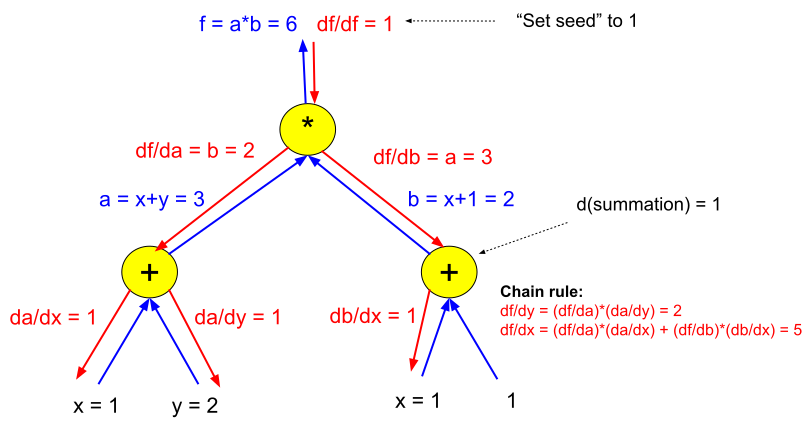
\includegraphics[scale=0.5]{img/slide/reversediff.png}
        \label{fig:reversediff}
    \end{figure}
\end{frame}

\begin{frame}{Code example}
\fontsize{7}{6}\selectfont
    AD usage example:
    \begin{figure}[H]
        \centering
            \includegraphics[scale=0.35]{img/slide/autodiff_julia.png}
        \label{fig:reversediff}
    \end{figure}
    
    Usage for optimization example:
    \begin{figure}[H]
        \centering
            \includegraphics[scale=0.27]{img/slide/autodiff_julia_opt.png}
        \label{fig:reversediff}
    \end{figure}
\end{frame}


%\subsection{"Differentiation" overview}
%\subsection{Forward mode}
%\subsection{Reverse mode}
%\subsection{Julia example}


\begin{frame}{References}
\fontsize{7}{6}\selectfont
\begin{itemize}
    \item [1.] U. Hager-Roiser. The potential energy surface of hydrogen clusters. MA thesis. University of Vienna, 2020.
    \item [2.] C. M. R. Rocha and A. J. C. Varandas. A general code for fitting global potential energy surfaces via CHIPR method: Direct-Fit Diatomic and tetratomic molecules. In: Computer Physics Communications 258 (2021), p. 107556. issn: 0010-4655. doi: 10.1016/j.cpc.2020.107556.
    \item [3.] Jörg Behler. Neural network potential-energy surfaces in chemistry: a tool for large-scale simulations. In: Phys. Chem. Chem. Phys. 13 (40 2011), pp. 17930–17955. doi: 10.1039/C1CP21668F.
    \item [4.] Atilim Gunes Baydin, Barak A. Pearlmutter, Alexey Andreyevich Radul, Jeffrey Mark Siskind. Automatic differentiation in machine learning: a survey. The Journal of Machine Learning Research, 18(153):1--43, 2018.
    \item [5.] Jeff Bezanson, Alan Edelman, Stefan Karpinski, and Viral B. Shah. 2017. Julia: A fresh approach to numerical computing. SIAM Rev. 59, 1 (2017), 65–98.
\end{itemize}
    
\end{frame}



\end{document}